% Chapter 7

\chapter{Evaluations} % Main chapter title

\label{eval} % For referencing the chapter elsewhere, use \ref{Chapter1} 

\lhead{Chapter 7. \emph{Evaluations}} % This is for the header on each page - perhaps a shortened title
\doublespacing
\setlength{\parindent}{1cm}
%\section{Conclusion}
%
%\section{Future Work}
%
%\subsection{Summarizing Event Related Content}
%
%\subsection{Identifying Insightful Opinionated Content Related to Events}
%
%\subsection{Event Topic Modeling}
%
%\subsection{Event-specific Recommendations}
%
%\subsection{Distributed Processing of EventIdentityInfoGraph}
%
%\subsection{Event Ontology for Social Media}

\section{Evaluation Baselines}

In order to evaluate the performance of \textit{EventIdentityInfoRank} we selected six different techniques that acted as our baselines. The six techniques along with their brief explanation and the reason behind their choice is discussed below.

\begin{enumerate}
\item \textbf{LexRank} - LexRank is a popular graph based algorithm commonly used in summarization of textual documents \cite{erkan2004lexrank}. It uses a stochastic graph-based method for computing the relative importance of textual units for Natural Language Processing. The task of extractive text summarization is based on the concept of identifying the most important sentences in a document or a set of documents. Importance is defined in terms of the presence of particular important words or in terms of similarity to a centroid pseudo-sentence. LexRank, computes sentence importance based on the concept of eigenvector centrality in a graph representation of sentences. In this model, a connectivity matrix based on intra-sentence cosine similarity is used as the adjacency matrix of the graph representation of sentences. We implement the LexRank algorithm using an open-source python module named sumy\footnote{\tiny https://pypi.python.org/pypi/sumy/0.1.0}, and rank the event related tweets considering them as individual sentences.

The objective of ranking natural language sentences in terms of their importance, makes it very similar to the \textit{EventIdentityInfoRank} algorithm as proposed in this dissertation for the purpose of ranking tweets instead of textual documents. \textit{EventIdentityInfoRank}, additionally ranks other units of information such as hashtags, text units, users and URLs, simultaneously, and does not takes into account the similarity of the tweets with a centroid pseudo-tweet. 

\item \textbf{TextRank} - TextRank is another popularly used technique used for summarization of textual documents \cite{Mihalcea2004}.  It is also a graph-based
ranking model for text processing, that can be successfully used in natural language
applications. The mechanism of its working is very similar to PageRank. However, instead of ranking web pages based on their linking structure, it ranks text units based on their linking structure. It can be used for identifying salient sentences as well as key words of a document. Its objective of identifying key words and important sentences is also similar to our objective of finding important tweets.

In our implementation, we modified the algorithm in order to make it suitable for our context. Apart from creating heterogeneous relationships in \textit{EventIdentityInfoGraph} we also created homogeneous relationships between the \textit{event identity information units}. Cosine similarity ($ \ge 0.10$) was used as the measure of relatedness between tweets, and the association scores of the hashtags, text units, users and URLs were based on their co-occurrence normalized between 0 and 1. The users were associated whenever they mentioned each other in the tweets, and the association score was measured by the number of mentions normalized between 0 and 1.


\item \textbf{Centroid} - Centroid is one of the techniques that was previously used in the literature for solving a part of our problem that ranks tweets. The technique is used for identifying high quality informative and useful tweets related to an event   \cite{becker2011selecting}. In order to implement it as a baseline we considered the tweets for the event in the given time period as one cluster. After preprocessing the tweets, we calculated the centroid of the cluster and ordered the tweets in the decreasing order of their similarities with the centroid.

\item \textbf{SeenRank} - SeenRank is a proprietary algorithm commercially used by Seen.co for generating event summaries and highlights from Twitter. We considered \textit{SeenRank} as the state-of-the-art technique. Although the true working of the algorithm is unknown, yet the task that the algorithm achieves is similar to the task of \textit{EventIdentityInfoRank}. In order to use this technique as one of our baselines. we also collected the tweets about the events tracked by our framework from Seen.co. The collection task was achieved using their API found at http://developer.seen.co/, and a freely available python wrapper pySeen\footnote{https://github.com/dxmahata/pySeen}, for collecting data from Seen.co. Each tweet collected from the website has a score assigned to it using SeenRank. We use this score for arranging the tweets in descending order. The ordering of the tweets were confirmed from the company's co-founder in order to be sure that greater score reflects higher ranking.



\item \textbf{RTRank} - Number of retweets is a good measure of popularity of a tweet and is also used by Twitter for ranking its search results. It is also commonly used by other paltforms for ranking tweets as already pointed out in Chapter \ref{review}. Therefore, we also considered tweets ordered in decreasing order of number of retweets as one of our baselines. We name this scheme as RTRank.

\item \textbf{Logistic Regression Model} - This technique is the logistic regression model that we implemented for initializing the informativeness score of the tweets in the `Event Information Quality' component. The generic informativeness score assigned by the logistic regression model is different from the final event-specific informativeness score assigned by \textit{EventIdentityInfoRank}. Also the logistic regression model acts as a good representative of supervised approaches. We explain this with an example.

On manually analyzing the informative tweets we tried to assess if it is good enough to train a classifier for detecting informative tweets for an event in order to identify valuable event-specific information. Although the tweets on which we trained our logistic regression model were related to events yet we came across tweets like, \textit{RT @BFDealz: http://t.co/TSJAigrVJI WHEELS SUPER TREASURE HUNT SUPERIZED HARLEY DAVIDSON FAT BOY LONG CARD 2014 \#cpac2014 \#sxsw}, which were classified as informative, even when it did not contain any event-specific information. 

This was probably because of the choice of features for the model, which were generic and not event-specific. The model did not take into account the presence of features that were popular and specific to the events, like popular hashtags, text units, etc. Popularity alone might not work as it is often mis-used by the spammers. It is also challenging to come up with a list of such event-specific features. Moreover, if one can compile such a list then it would be difficult to set thresholds on each such feature in order to qualify it as event-specific. Also, a supervised classification model does not have the ability to simultaneously rank tweets, hashtags, text units, URLs and users in terms of event-specific informativeness. After going through the existing literature we assume that the challenges discussed above would be a shortcoming of any supervised model and there is a need for an alternative feasible approach. It is also difficult to predict the event-specific informativeness in the URLs shared along with the tweets, as it might be necessary to analyze the content pointed to by the URLs. Also, not all the URLs contain text. They might be images or videos providing valuable information about an event. This motivated us to devise a novel framework that solves all the above problems.


Therefore, we considered the model as one of our baselines in order to make sure that our \textit{EventIdentityInfoRank} improves upon the initial generic informativeness score already assigned to the tweets at the start of the iteration and assigns event-specific informativeness scores on convergence. In other words the tweets having high score after the final ranking are more useful and informative than the initial ranking obtained using the logistic regression model.

\end{enumerate}


Due to unavailability of proper baseline techniques for ranking hashtags, text units, URLs and users in terms of event-specific informativeness we do not compare the results obtained for them with any other approach. However, we report their average scores and sample results. Please refer the previous chapter for the sample results.

\section{Evaluation Setup and Objectives}
We evaluated the rankings obtained using \textit{EventIdentityInfoRank} on the  datasets (refer Chapter \ref{eiim}, `Event Reference Collection' component), collected for events: ``Millions March NYC'' and ``Sydney Siege Crisis", by comparing its performance with the selected baselines. A subset of tweets for each event for a given time period (one hour) was selected. The choice of the time period was made on the basis of the interesecton of the time period of the tweets collected by us and that provided by Seen for the same event. There were 21641 tweets for Millions March NYC and 37429 tweets for Sydney Siege, respectively. We obtained the ranked tweets for all the seven approaches. For all the approaches except \textit{SeenRank} the tweets were sorted in decreasing order on the basis of the ranking scores as the primary key and time of posting as the secondary key. This was done in order to get the most informative yet recent tweets at the top of the order. For \textit{SeenRank} we sorted the tweets in terms of the scores assigned to them by Seen, as showing recent informative tweets for an event is one of the features of their platform.

We then followed a standard user evaluation approach to judge the event-specific informativeness of ranked tweets and also the hashtags, text units, URLs, and users.  A team of three independent annotators comprising of graduate students, having taken the course of Information Retrieval, were assigned the task of annotation. Necessary background of the events were given to the annotators along with suitable resources for learning more about the events. Next, we present the annotation schemes.

\begin{table}[htbp]
\centering
\caption{Avg IIC scores and total avg scores of annotations for Millions March NYC event.}
\label{avgiicMillionsMarchNyc}
\begin{tabular}{|c|c|c|}
\hline
\textbf{\begin{tabular}[c]{@{}c@{}}Millions March \\ NYC\end{tabular}} & \textbf{IIC} & \textbf{\begin{tabular}[c]{@{}c@{}}Total Avg \\ Score (1-3)\end{tabular}} \\ \hline
\textbf{\begin{tabular}[c]{@{}c@{}}Top 50 event-specific\\ informative Hashtags\end{tabular}} & 0.786 & 1.980 \\ \hline
\textbf{\begin{tabular}[c]{@{}c@{}}Top 50 event-specific\\ informative Text Units\end{tabular}} & 0.880 & 1.320 \\ \hline
\textbf{\begin{tabular}[c]{@{}c@{}}Top 50 event-specific\\ informative URLs\end{tabular}} & 0.926 & 2.560 \\ \hline
\textbf{\begin{tabular}[c]{@{}c@{}}Top 50 event-specific\\ informative Users\end{tabular}} & 0.700 & 2.386 \\ \hline
\textbf{\begin{tabular}[c]{@{}c@{}}Top 100 event-specific\\ informative Tweets\end{tabular}} & 0.760 & 2.59 \\ \hline
\end{tabular}
\end{table}

\begin{table}[htbp]
\centering
\caption{Avg IIC scores and total avg scores of annotations for Sydney Siege event.}
\label{avgiicSydneySiege}
\begin{tabular}{|c|c|c|}
\hline
\textbf{Sydney Siege} & \textbf{IIC} & \textbf{\begin{tabular}[c]{@{}c@{}}Total Avg\\ Score (1-3)\end{tabular}} \\ \hline
\textbf{\begin{tabular}[c]{@{}c@{}}Top 50 event-specific\\ informative Hashtags\end{tabular}} & 0.880 & 2.027 \\ \hline
\textbf{\begin{tabular}[c]{@{}c@{}}Top 50 event-specific\\ informative Text Units\end{tabular}} & 0.986 & 1.487 \\ \hline
\textbf{\begin{tabular}[c]{@{}c@{}}Top 50 event-specific\\ informative URLs\end{tabular}} & 0.893 & 2.413 \\ \hline
\textbf{\begin{tabular}[c]{@{}c@{}}Top 50 event-specific\\ informative Users\end{tabular}} & 0.646 & 2.353 \\ \hline
\textbf{\begin{tabular}[c]{@{}c@{}}Top 100 event-specific\\ informative Tweets\end{tabular}} & 0.83 & 2.62 \\ \hline
\end{tabular}
\end{table}

\subsection{Tweet Annotation} 
The ranked tweets were annotated on an event-specific informativeness-scale of 1 to 3 by the three independent annotators. We provide sample tweets for each of them taking the Sydney Siege event as our example. 

\begin{itemize}
\item The value of 1 was assigned to tweets that does not contain any event related information (for e.g. \textit{SteveSmith becomes Australias 45th Test captain http://t.co/nYh9DqRXxh \#sydneysiege \#MartinPlace Lindt \#MYEFO \#siege Ray Hadley Muslims ISIS}). 
\item Value of 2 was assigned to tweets that were related to the event yet they did not provide useful event-specific information (for e.g. \textit{RT @TheDavidStevens: It wasn't just the policeman grabbing that girl in his arms, it was every Australian watching on too \#sydneysiege} ). 
\item A value of 3 was assigned to tweets that not only provided useful event-specific informative content but also led the user to more detailed information following the URLs mentioned in the tweet (for e.g. \textit{RT @FoxNews: MORE: Police confirm 3 hostages escape Sydney cafe, unknown number remain inside http://t.co/pcAt91LIdS \#Sydneysiege}).  
\end{itemize}



The annotators assigned scores to top 100 tweets ranked according to each of the seven strategies. Thereafter, we computed \textit{Inter Indexer Consistency} (IIC) values \cite{rolling1981indexing} for the annotations of the two datasets. The average IIC scores obtained for the two events are are shown in Table \ref{avgiicMillionsMarchNyc} and Table \ref{avgiicSydneySiege}, respectively. The IIC values for both the events fall in the acceptable range of accuracy of annotations. A tweet might be assigned three different scores by the annotators. In that scenario we find the average of the three scores and round it off to the smallest positive integer and assign a single score to each tweet. We also report the total average scores for top 100 tweets for both the events in the tables. 

\subsection{Hashtags, Text Units and URL Annotations}
A similar annotation strategy was taken for annotating the top 50 hashtags, text units and URLs obtained using \text{EventIdentityInfoRank}. For hashtags and text units the annotators were asked to look at the tweets that consisted them. Following strategy was followed for scoring.

\begin{itemize}
\item If the tweets containing them primarily led to event-specific informative content then a score of 3 was assigned.

\item If the tweets containing them led to related but not so informative content about the event then they were assigned a score of 2.

\item Hashtags and text units that were irrelevant and did not lead to any event related content, were assigned a score of 1.
\end{itemize}

Similarly, the annotators visited the links for each URL, and based on the content they assigned them a score between 1-3. If the URLs were videos and images, then they further visited the tweet containing them in order to understand the context and scored them accordingly. Table \ref{avgiicMillionsMarchNyc} and Table \ref{avgiicSydneySiege} shows their average IIC scores and total average scores for top 50 ranks. 

\subsection{User Annotations} 
For annotating users we selected 5 random tweets for each of the top 50 users ranked according to \textit{EventIdentityInfoRank}. An user was assigned a score of 3 if more than three of his tweets out of five got a score of 3 in the event-specific informativeness scale as already explained earlier. If three of his tweets get a score of 3 then the user gets a score of 2. Otherwise, a score of 1 is assigned to the user. Table \ref{avgiicMillionsMarchNyc} and Table \ref{avgiicSydneySiege} shows average IIC scores and total average scores for top 50 users.

 
\subsection{NDCG@n and Precision@n}
After being assured about consistency and accuracy of annotations, we moved to compute the \textit{Normalized Discounted Cumulative Gain} (NDCG) \cite{jarvelin2002cumulated} and Precision \cite{baeza1999modern} values at each of the hundred recall levels. The NDCG values consider both the position and event-specific informativeness scores of the tweets. The NDCG value up-to position $p$ in the ranking is given by equation \ref{eq62}, where $DCG_{p}$ denotes the \textit{discounted cumulative gain up-to position p} and is calculated using equation \ref{eq61}, and $IDCG_{p}$ denotes the \textit{ideal discounted cumulative gain} value till position $p$ in the ranking, or in other words the maximum possible $DCG_{p}$ value till position $p$. $rel_{i}$ denotes the graded relevance of the result at position $i$. In the context of our evaluation $rel_{i}$ represents the average rounded score in the scale of (1-3) that has been assigned by the annotators to the tweet at position  $i$ in the ranked list of top 100 tweets.

\begin{equation}
\label{eq61}
DCG_{p} = \sum_{i=1}^{p}\frac{2^{rel_{i}}-1}{log(i+1)}
\end{equation}

\begin{equation}
\label{eq62}
nDCG_{p} = \frac{DCG_{p}}{IDCG_{p}} 
\end{equation}

Precision@n is measured using equation \ref{eq63}. A tweet was considered to be relevant if it has a score of either 3 or 2 and was considered irrelevant if it has a score of 1.

\begin{equation}
\label{eq63}
\frac{No.\,of\, relevant\, tweets\, at\, position\, n}{n}
\end{equation}

NDCG@n and Precision@n values were calculated for all the seven approaches for each of the datasets. Figures \ref{millionsmarchndcg} and \ref{sydneysiegendcg} shows the NDCG curves for all the seven approaches on the Millions March NYC and the Sydney Siege events, respectively, for up-to 20 recall levels. Tables \ref{sydneysiegendcgtable} and \ref{sydneysiegeprecisiontable} presents the NDCG@n values and Precision@n values for different recall levels upto 100 for the Sydney Siege Crisis event. Similarly, Tables \ref{millionsmarchndcgtable} and \ref{millionsmarchnycprecisiontable} presents the NDCG@n values and Precision@n values for different recall levels upto 100 for the Millions March Nyc event.It is quite evident from the figures and the tables that EventIdentityInfoRank approach outperforms all the baselines including the state-of-the-art approach of \textit{SeenRank} in gaining event-specific information.



\begin{figure}[htbp]
\centering
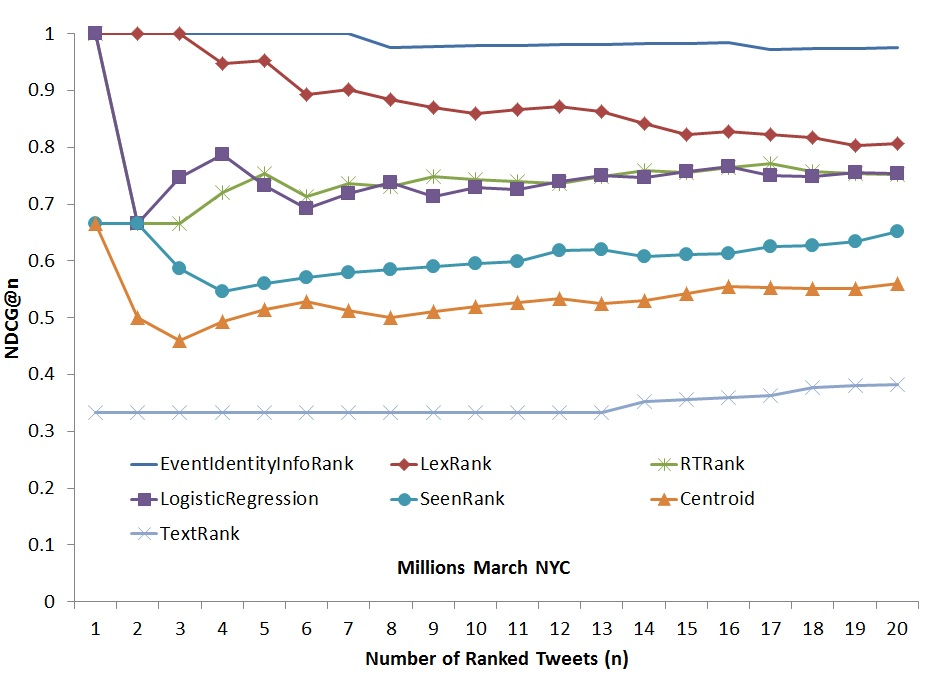
\includegraphics[height=4.5in,width=6in]{Figures/EventIdentityInfoRankPerformanceMillionsMarchNyc.jpg}
\caption{Performance comparison of ranking techniques using NDCG scores.}
\label{millionsmarchndcg}
\end{figure}

\begin{figure}[htbp]
\centering
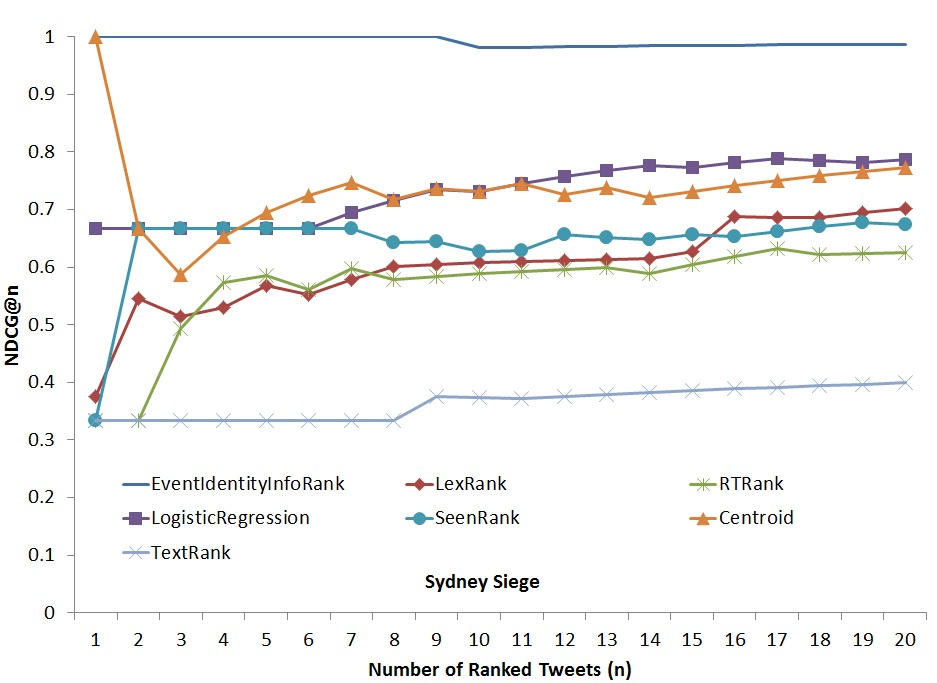
\includegraphics[height=4.5in,width=6in]{Figures/EventIdentityInfoRankPerformanceSydneySiege.jpg}
\caption{\small Performance comparison of ranking techniques using NDCG scores.}
\label{sydneysiegendcg}
\end{figure}






\begin{figure}[htbp]
\centering
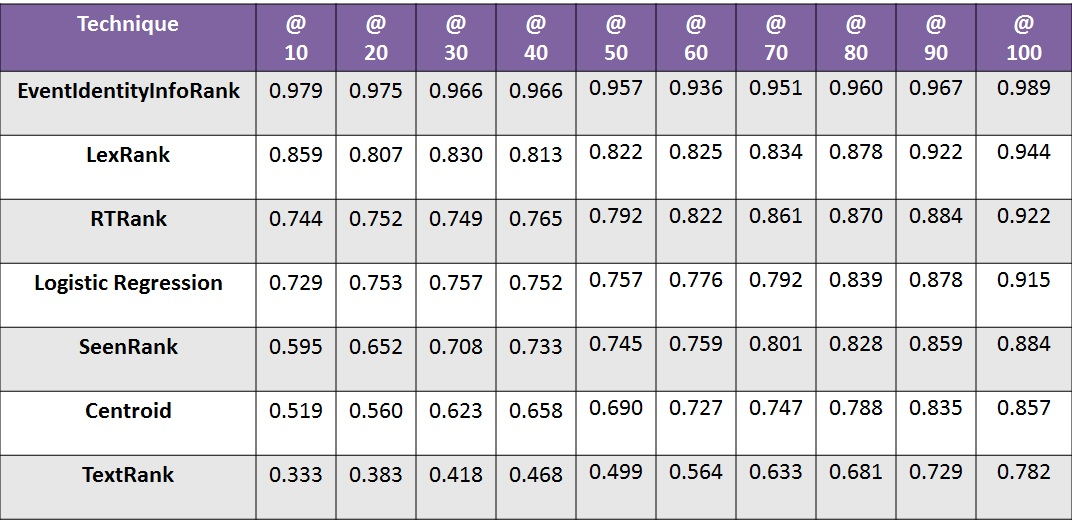
\includegraphics[height=3in,width=5.5in]{Figures/MillionsMarchNycCorrectedNDCG.jpg}
\caption{Performance comparison of ranking techniques using NDCG scores.}
\label{millionsmarchndcgtable}
\end{figure}

\begin{figure}[htbp]
\centering
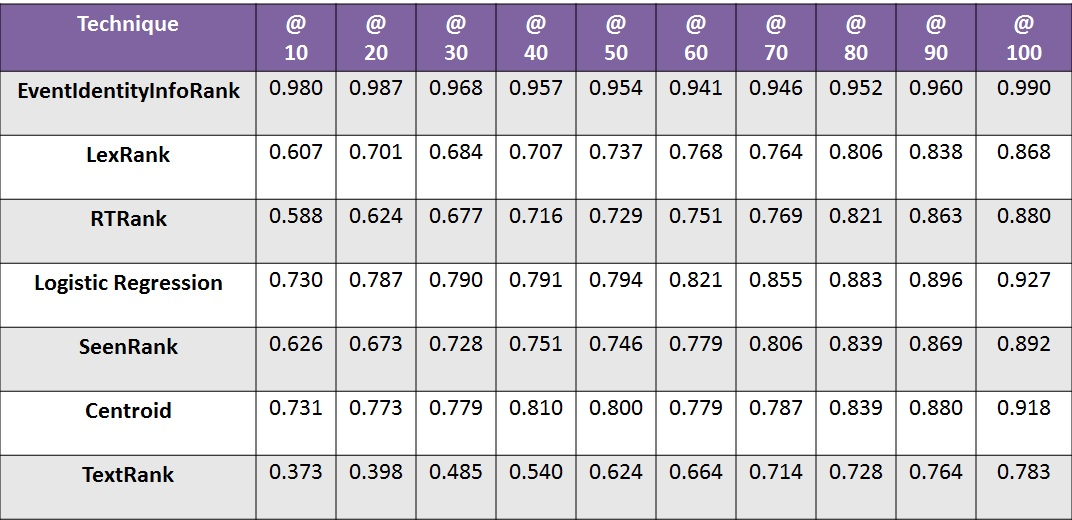
\includegraphics[height=3in,width=5.5in]{Figures/sydneysiegecorrectedndcg.jpg}
\caption{Performance comparison of ranking techniques using NDCG scores.}
\label{sydneysiegendcgtable}
\end{figure}

\begin{figure}[htbp]
\centering
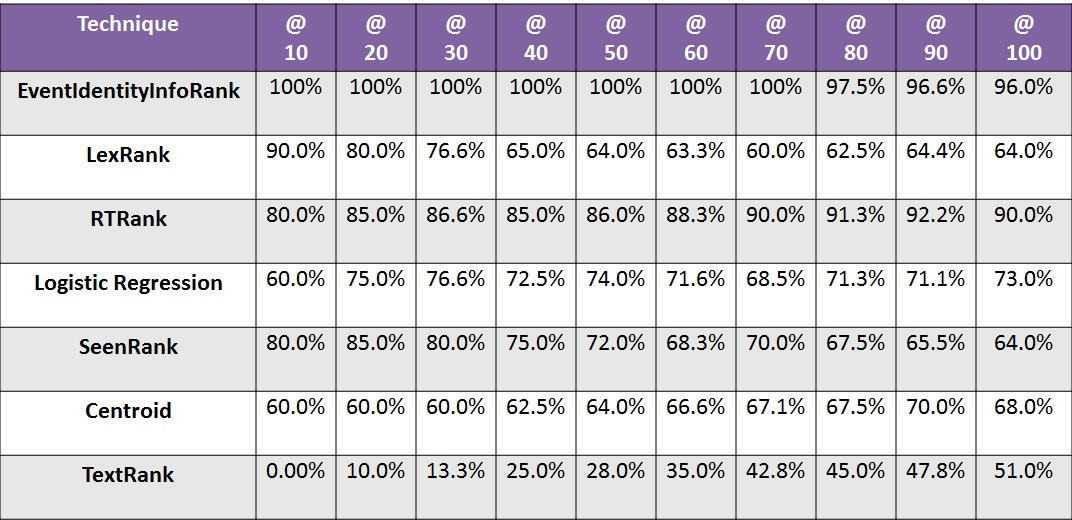
\includegraphics[height=3in,width=5.5in]{Figures/MillionsMarchNycCorrectedPrecision.jpg}
\caption{Performance comparison of ranking techniques using precision scores.}
\label{millionsmarchnycprecisiontable}
\end{figure}

\begin{figure}[htbp]
\centering
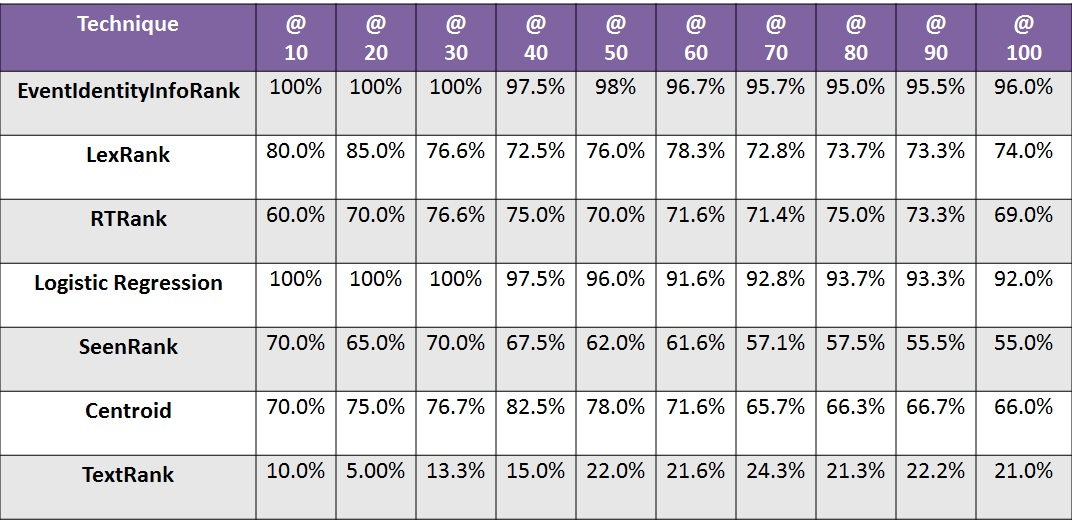
\includegraphics[height=3in,width=5.5in]{Figures/sydneysiegeprecisioncorrected.jpg}
\caption{Performance comparison of ranking techniques using precision scores.}
\label{sydneysiegeprecisiontable}
\end{figure}

On considering only the top 10 tweets we observed a substantial information gain of our algorithm over the state-of-the-art (\textit{SeenRank}) and the baseline that performed second best for both the events. On comparing the values of NDCG@10 for the two events we found that our algorithm performs 13.96\% (Millions March NYC) and 34.07\% (Sydney Siege) better than the second best baseline technique, in identifying event-specific informative tweets. When compared with \textit{SeenRank}, our algorithm was 64.53\% (Millions March NYC) and 56.59\% (Sydney Siege) better. 

We also reasoned about the poor performance of \textit{TextRank} in both the events. Since \textit{TextRank} allowed random walks between homogeneous nodes, the strong association of non-informative nodes with the informative ones might have lowered the final scores of the informative nodes. The strong association of non-informative nodes with informative ones can be attributed to the spamming activity as already explained earlier Chapter \ref{review}, Section \ref{veracity} This also proves that our framework is robust against spams and is very effective in identifying the most informative content related to events from the noisy stream of tweets in Twitter. 

